% ----------------------- TODO ---------------------------
% Diese Daten müssen pro Blatt angepasst werden:
\newcommand{\NUMBER}{6}
\newcommand{\EXERCISES}{5}
% Diese Daten müssen einmalig pro Vorlesung angepasst werden:
\newcommand{\COURSE}{Grundlagen der Digitaltechnik}
\newcommand{\TOPIC}{Programmable Logic}
\newcommand{\DATE}{25.05.2022}
% ----------------------- TODO ---------------------------

\documentclass[a4paper]{scrartcl}

\usepackage[utf8]{inputenc}
\usepackage[ngerman]{babel}
\usepackage{amsmath}
\usepackage{amssymb}
\usepackage{fancyhdr}
\usepackage{color}
\usepackage{graphicx}
\usepackage{lastpage}
\usepackage{listings}
\usepackage{tikz}
\usepackage{pdflscape}
\usepackage{subfigure}
\usepackage{float}
\usepackage{polynom}
\usepackage{hyperref}
\usepackage{tabularx}
\usepackage{forloop}
\usepackage{geometry}
\usepackage{listings}
\usepackage{fancybox}
\usepackage{tikz}
\usepackage{algpseudocode,algorithm,algorithmicx}

%Definiere Let-Command für algorithmen
\newcommand*\Let[2]{\State #1 $\gets$ #2}

\input kvmacros

%Größe der Ränder setzen
\geometry{a4paper,left=3cm, right=3cm, top=3cm, bottom=3cm}

%Kopf- und Fußzeile
\pagestyle {fancy}
\fancyhead[L]{\COURSE}
\fancyhead[R]{\DATE}

\fancyfoot[L]{}
\fancyfoot[C]{}
\fancyfoot[R]{Seite \thepage /\pageref*{LastPage}}
\setlength{\parindent}{0pt}

%Formatierung der Überschrift, hier nichts ändern
\def\header#1#2{
  \begin{center}
    {\Large Labor #1: \TOPIC}\\
    {(Datum #2)}
  \end{center}
}


\begin{document}


\header{Nr. \NUMBER}{\DATE}


\section*{Aufgabe 1: Programmable Logic}
Logisim hat in seinen Bibliotheken zwei Arten  von PLAs (Programmable Logic Arrays).
Der PLA-Block in ``Input/Output Extra'' verhält sich wie ein PLA, das in der Vorlesung beschrieben wurde. Fügt man den Baustein ein,
macht einen Rechts-Click $\rightarrow$ ``Edit Contents'' dann öffnet sich ein Editor, welcher genau die AND/ODER Matrix aus der Vorlesung darstellt.
Ein Click auf die Kreuzungen der Leitungen verbindet diese.
\begin{figure}[h]
  \centering
  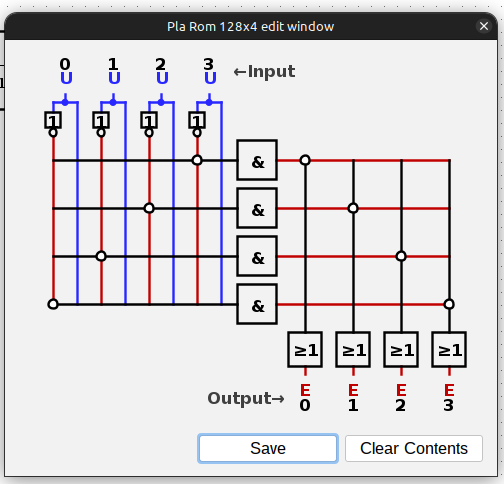
\includegraphics[width=6cm]{pla_logisim.png}
\caption{PLA Editor}
\end{figure}

Ein weiterer Block, welcher von Logisim PLA genannt wird, ist im Reiter ``Gates'' zu finden. Dieser PLA-Block stellt aber eigentlich
eine Look-Up Table (LUT) dar. In dem zugehörigen Editor kann man direkt die Look-Up Table eintragen.


\begin{figure}[h]
  \centering
  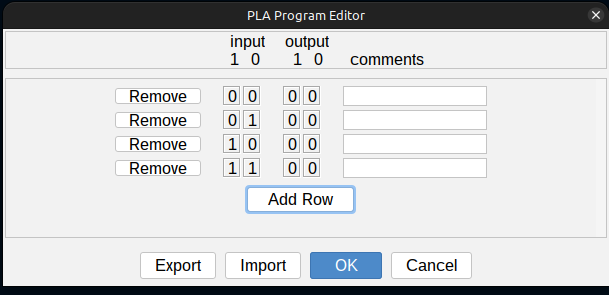
\includegraphics[width=7cm]{lut_editor.png}
\caption{PLA (LUT) Editor}
\end{figure}

\subsection*{a) Revisiting BCD27Seg}
Im letzten Labor wurde für den BCD to 7 Segments Converter eine Wahrheitstabelle aufgestellt. Nutze diese 
Wahrheitstabelle, um den Converter mit den beiden Arten von ``PLA'' Blöcken zu implementieren.\\

\subsubsection*{i.) Look-Up Table}
In den Look-Up Table Baustein (PLA in Gates)  kann die Wahrheitstabelle direkt eingetragen werden.\\

\textbf{Hinweis:}
\begin{itemize}
  \item Der LUT Editor öffnet sich per Rechts-Click auf das Bauteil $\rightarrow$ Edit PLA Program
\end{itemize}

\subsubsection*{ii.) PLA}
Bei dem eigentlichen PLA Baustein können verschiedenste Min-Terme auf einem ODER für einen bestimmten Ausgang zusammengeschaltet werden (s. Abbildung 1).
Es muss daher ermittelt werden wie viele einzelne Min-Terme der komplette BCD to 7 Segments Converter hat (jeder Min Term kann auf beliebig viele
ODER Gates geschalten werden, daher braucht man diese nicht doppelt). Die Anzahl der Min-Terme bestimmt dann die Anzahl der AND Gates (einstellbar).\\


\textbf{Hinweise:}
\begin{itemize}
  \item Der PLA Editor öffnet sich per Rechts-Click auf das Bauteil $\rightarrow$ Edit Contents
  \item Bevor die Logik implementiert wird, sollte herausgefunden werden, wie die numerierten Ein-/Ausgänge im Editor auf die Ein-/Ausgangspins mappen. Dies ist etwas kontraintuitiv.
\end{itemize}

\subsubsection*{iii.) Test}
Baue mit beiden erstellten Blöcken die 4-Stellige Anzeige von letzter Woche nach, um die jewiligen Implementierungen zu testen.

\section*{Aufgabe 2: Logic with ROM}
ROM-Bausteine (Read only Memory) sind Speicherbausteine, welche in der Fertigung einmalig mit einem Inhalt beschrieben werden und danach nicht mehr veränderbar sind.
Auch mit Speicherbausteinen kann Logik implementiert werden. Die Bausteine funktionieren so:
\begin{itemize}
  \item An den Eingang wird eine n-Bit breite Addresse angelegt
  \item Der Baustein gibt den einprogrammierten Inhalt der Speicherzelle von der angelegten Addresse zurück. Dieser Inhalt kann m-Bit breit sein.
\end{itemize}

Es soll nun ein Addierer, Multiplizierer und Dividierer mithilfe dieser ROM-Bausteine implementiert werden (Logisim: Memory $\rightarrow$ ROM), welcher
jeweils 2 2-Bit Zahlen als Eingang hat und eine 4-Bit Zahl als Ergebnis zurückliefert. Beantworte zuerst die Fragen, bevor mit der 
Implementierung angefangen wird.\\

\textbf{Fragen:}
\begin{itemize}
  \item Wie breit muss die Addressleitung des Bausteins sein? Wie viele Speicherzellen besitzt dieser dann?
  \item Wie breit muss eine einzelne Speicherzelle sein?
  \item Wie viele Bits kann der Baustein insgesamt speichern?
  \item Kann man allgemein sagen wie Address- und Speicherzellenbreite mit den Ein- und Ausgängen einer Logikschaltung zusammenhängen?
\end{itemize}

Implementiere nun die drei Schaltungen. Den Inhalt der Speicherzellen
des ROMs kann man mit Rechts-Click auf das Bauteil $\rightarrow$ Edit Contents bearbeiten.\\

\textbf{Hinweise:}
\begin{itemize}
  \item Integer-Division funktioniert so, dass ein vermeintlicher Rest einer Division einfach ``verloren'' geht.
  \item Um Dinge nicht übermäßig zu verkomplizieren, gib einfach 0 zurück, wenn durch 0 geteilt werden würde.
\end{itemize}

\section*{Aufgabe 3: LED-Matrix}
In Logisim gibt es im ``Input/Output'' Reiter eine LED-Matrix. Die LED Matrix hat einstellbar viele Pixel, welche alle einzeln ein- und ausgeschaltet werden können (vgl. Abbildung 3).
Es kann umgeschalten werden, ob reihen- oder spaltenweise addressiert werden soll (``Input Format'').
\begin{figure}[h]
  \centering
  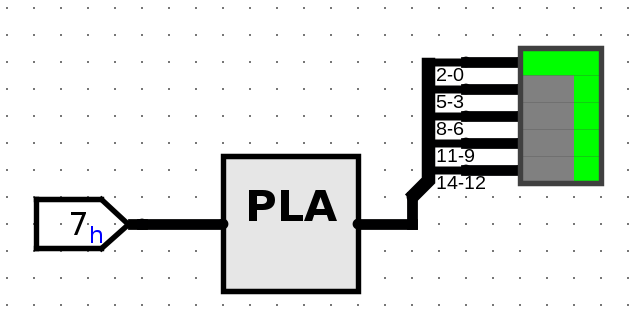
\includegraphics[width=6cm]{LEDMatrix.png}
\caption{LED Matrix}
\end{figure}


\textbf{Aufgaben:}
\begin{enumerate}
  \item Implementiere mit Logikbausteinen deiner Wahl (Gatter-Logik, PLA, ROM...) einen Converter, welcher einen 4-Bit BCD codierten Eingang, so umwandelt, dass eine 5$\times$3 LED Matrix die Zahl als Dezimalzahl
  anzeigt.
  \item Baue nach einem Funktionstest des Converters die Digitaluhr von letzter Woche mit den LED-Matrix Displays nach (eine 5$\times$3 LED Matrix soll eine 7 Segment Anzeige ersetzen).
\end{enumerate}



\end{document}
%%% Local Variables:
%%% mode: latex
%%% TeX-master: t
%%% End: